\documentclass[11pt]{article}
\usepackage[utf8]{inputenc}
\usepackage[margin=0.5in]{geometry}
\usepackage{graphicx}
\begin{document}

\begin{center}
    CS310 -- Assignment 423 -- Karl Ramberg
\end{center}

To test my Sudoku solver program I searched for a few easy and hard puzzles online. \texttt{sudoku.com} offered easy, medium, hard, and expert level puzzles so I tested one of each. Here are the results...

\begin{center}
    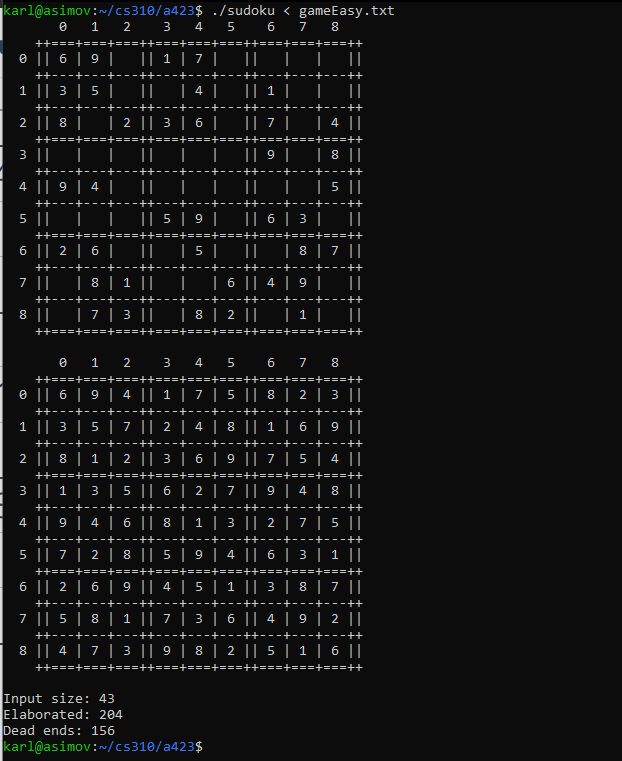
\includegraphics[width=0.75\textwidth]{easy.png} 
    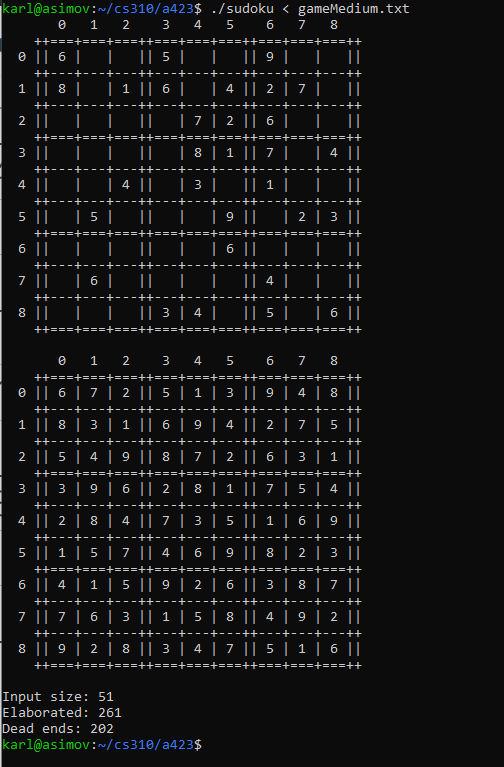
\includegraphics[width=0.75\textwidth]{medium.png} 
    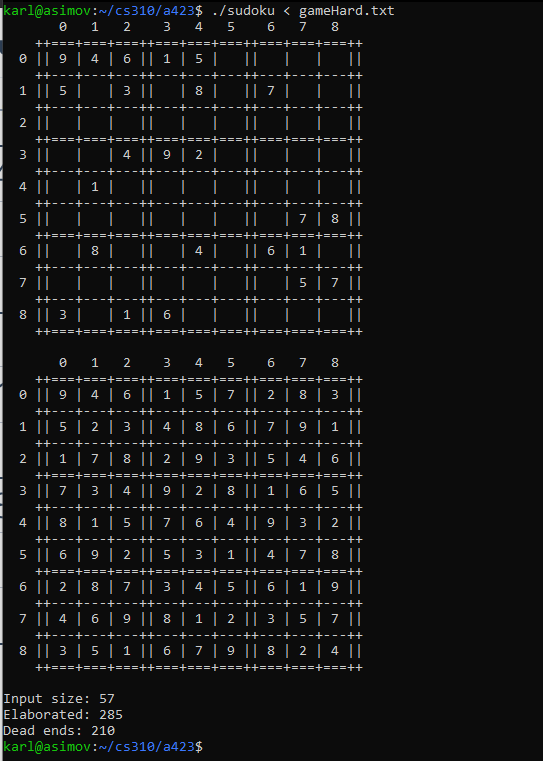
\includegraphics[width=0.75\textwidth]{hard.png}
    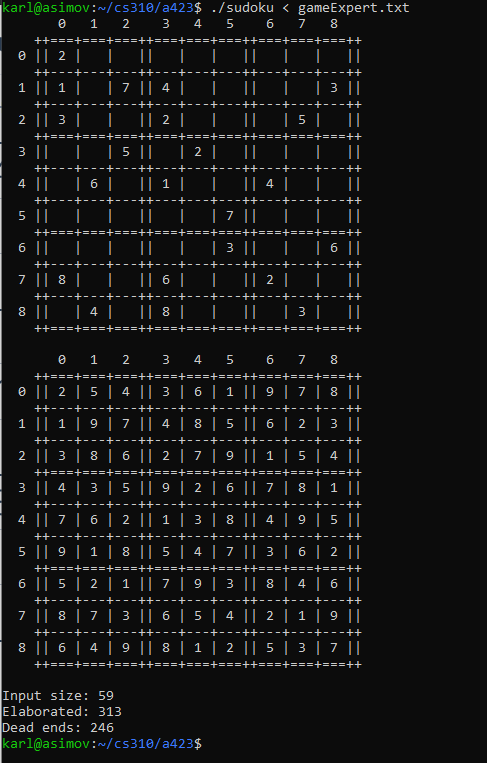
\includegraphics[width=0.75\textwidth]{expert.png}
\end{center}

Through this testing you can see that puzzles meant to be harder for humans are also hard for my Sudoku solver. The easy puzzle only took $204$ elaborated nodes while the expert took $313$. The easy puzzle had $156$ dead ends while the expert puzzle had $246$. The medium and hard puzzles we somewhere in between.

It's hard to tell how hard a sudoku will be to solve before you start working it, but the largest indicator seems to be how many cells are filled in to start. The expert puzzle had $22$ filled in to start while the easy one had $37$. This would make sense as an input size if we were to analyze this program fully. However, it maybe better represented as the number of empty cells to start -- this would give us the common correlation of basic operations increasing with input size.

This would mean that the hardest puzzle to solve would be an empty grid. This is the hardest puzzle for my program to solve that I found with my testing with $405$ elaborated nodes and $303$ dead ends.

\begin{center}
    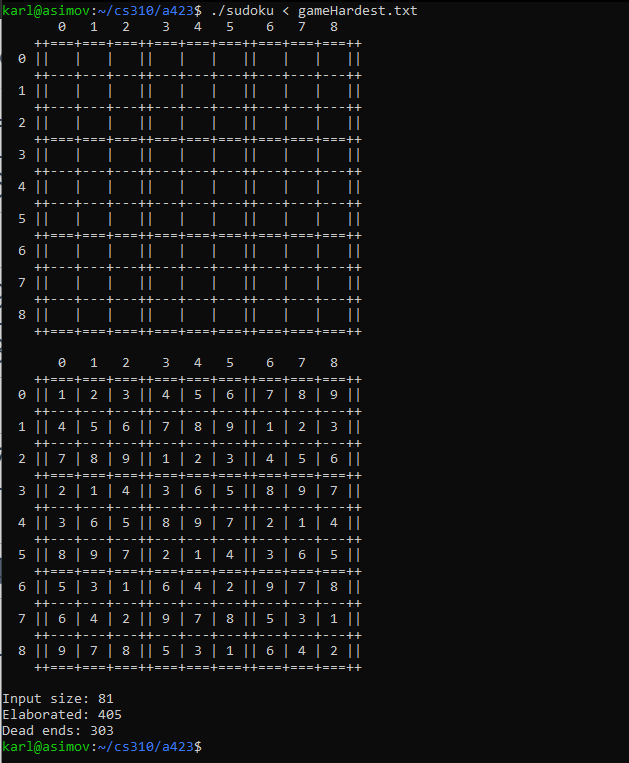
\includegraphics[width=0.75\textwidth]{hardest.png}
\end{center}
\end{document}